\chapter{Matrix Multiplication} \label{chap:sota2}

\section*{}
  
This chapter is about matrix multiplication algorithms. Two possible versions for the same problem are presented in the following sections. The last sections of this chapter is a recap of both algorithms. 

\section{Introduction}

In the state of the art regarding matrix multiplication, there is an abundance in algorithms trying to optimize these computational operations~\cite{Goto2008}~\cite{Yuster2005}, since it is used in, for instance, GPUs~\cite{Fatahalian2004}.
 
Two different algorithm versions for the same problem are presented because they are going to be used as mean to prove that, firstly, parallel code increases performance in a huge scale, and, secondly, parallel code made in an automatic way can have similar results as the same code being manually parallelized by an expert.

The first algorithm is the general and classic approach of the problem. The second algorithm is an enhanced version of the same algorithm but with a new perspective, taking advantages of the hardware components, such as cache memory.

\section{Classic Algorithm)}\label{sec:dialecto}


The classic version of this algorithm~\cite{Fatahalian2004}, computes the multiplication of two matrix with the same dimension as it follows:

\begin{equation}
C_{ij} = (AB)_{ij} = \sum_{k=0}^{n-1} a_{ik} b_{kj} = a_{i1} b_{1j} + ... + ai_{(n-1})b_{(n-1)j}
\end{equation}

\textbf{Where:}

\begin{description}
	\item [C_{ij}] Resulting matrix from matrix multiplication between A and B;
	\item [(AB)_{ij}] matrix multiplication between A and B;
	\item [n] Matrix size NxN;
	\item [a_{ik}] Element from line i and column k belonging to Matrix A;
	\item [b_{kj}] Element from line k and column j belonging to matrix B.
\end{description}

This algorithm multiplies the first line of matrix A for each column of matrix B, as it is presented in ~\ref{fig:esquemamult}

\begin{figure}[htb]
	\begin{center}
		\leavevmode
		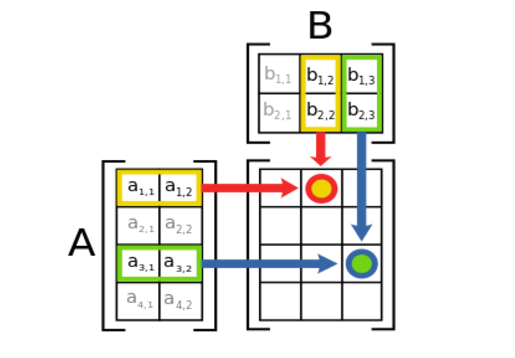
\includegraphics[width=0.7\textwidth]{esquemamult}
		\caption{Matrix multiplication between matrix A(4x2) and  B(2x3), representative matrices.}
		\label{fig:esquemamult}
	\end{center}
\end{figure}

So, the pseudo code used to implement~\ref{code:onmul} is the following:

\begin{lstlisting}
	for(i=0; i<n; i++) {	
		for( j=0; j<n; j++) {	
			for( k=0; k<n; k++) {	
				C[i][j]+= A[i][k] * B[k][j];
			}
		}
	}
\end{lstlisting}


\section{In Line Algorithm}

This algorithm version computes matrix multiplication differently comparing to the classic algorithm:

\begin{equation}
C_{ij} = (AB)_{ij} = \sum_{j=0}^{n-1} a_{ik} b_{kj} = a_{i1} b_{1j} + ... + ai_{(n-1})b_{(n-1)j}
\end{equation}

\textbf{Where:}

\begin{description}
	\item [C_{ij}] Resulting matrix from matrix multiplication between A and B;
	\item [(AB)_{ij}] matrix multiplication between A and B;
	\item [n] - Matrix size NxN;
	\item [a_{ik}] Element from line i and column k belonging to Matrix A;
	\item [b_{kj}] Element from line k and column j belonging to matrix B.
\end{description}

This algorithm multiplies an element form matrix A for the correpondent line of matrix B, as it is suggested in~\ref{fig:esquemamultline}:

\begin{figure}[htb]
	\begin{center}
		\leavevmode
		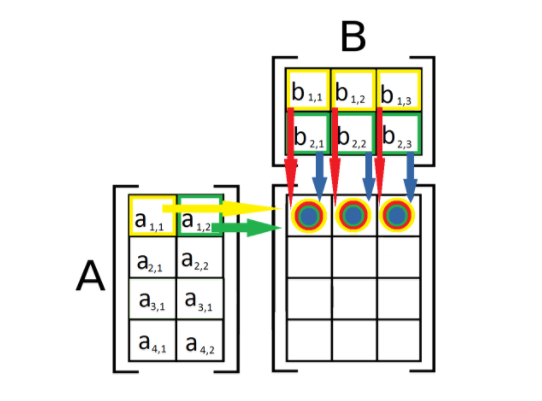
\includegraphics[width=0.7\textwidth]{esquemamultline}
		\caption{Matrix multiplication in line between matrix A(4x2) and  B(2x3), representative matrices.}
		\label{fig:esquemamultline}
	\end{center}
\end{figure}

So, the pseudo code used to implement~\ref{code:onmuline} is the following:

\begin{lstlisting}
for(i=0; i<n; i++) {	
	for( k=0; k<n; k++) {	
		for( j=0; j<n; j++) {	
			C[i][j]+= A[i][k] * B[k][j];
		}
	}
}
\end{lstlisting}

\section{Overview}

In terms of code implementation, the biggest difference in these two algorithms is in the permutation between the second and third inner \textit{for} loop, which, consequently, has an huge impact in performance~\cite{Lam}.

This slight alteration in the classic algorithm makes matrix multiplication in line much faster when implemented in an application. The way and order of the operations are made for this algorithm is what makes this algorithm better: the order the calculation is made takes advantage of what is preloaded in cache memory. By doing though, it reduces the number of times a cache miss happens, which, consequently, reduces the number of times information is replaced in cache memory, reducing the number of times memory cache is written, therefore, reducing the waiting time until cache memory has the required information, reducing the overall application time, which improves application performance.

However, the matrix multiplication in line algorithm is best suited  for long matrix sizes, for instances, if the matrices fit in cache memory, this algorithm, that reduces the number of cache memory swaps, makes almost no differences in overall performance.
